

The \texttt{Basilisk} code has been validated numerous time in previous numerical studies \todo{Add biblio}\citet{innocenti2020direct},\citet{popinet2018numerical}. 
Therefore,  in this section we start by presenting a brief comparison with previous numerical studies. 
Afterward we present a meticulous study focusing on the interfaces dynamics, by comparing our results with the experimental results of \citet{mohamed2003drop} 
To complete these valildation we present in \ref{ap:A} several classic cases analyzing :
(1) The mesh definition, (2) The statistical time convergence, (3) the number of particles on random array of droplets. 
 
\subsection{Fixed array of bubbles}
Objectives :
\begin{itemize}
    \item Mesh validation : our DNS Vs. DNS of \cite{esmaeeli1999direct}
\end{itemize}
From our knowledge, no simulations nor experimental results have been carried out for rising buoyant viscous drop. 
Therefore, instead we reproduced the well known ordered array simulation of \citet{esmaeeli1999direct} with Basilisk to validate the mesh definition.  
It consists in a 3-D buoyant ordered rising array of bubbles. 
In our notation the flow parameters of the simulation reads, 
\begin{align*}
    \mu_r = 10,
    && \rho_r = 10,
    && Bo = 1.8,
    && Ga = 28.37,
    && \phi = 0.125.
\end{align*}
\begin{figure}[h!]
    \centering
    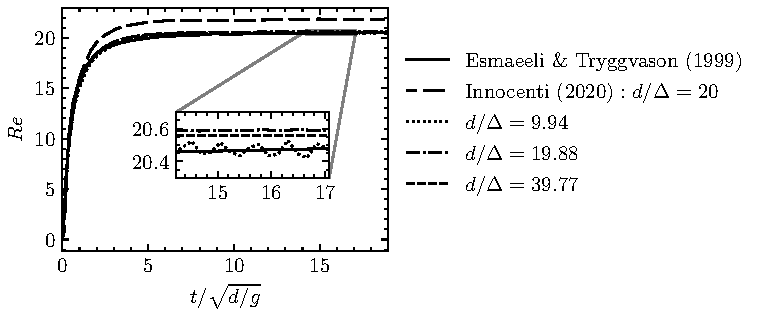
\includegraphics[height = 0.35\textwidth]{image/VALIDATION2.0/Loisy/Re.pdf}
    \caption{Time evolution of the Reynolds number based on the instentaneous volume averaged drift velocity, $Re(t) = \rho_fU d /\mu_f$, with $U(t) = (\Xavg{\textbf{u}_p} - \Xavg{\textbf{u}_c})\cdot \textbf{e}_y$ with $\phi = 0.1256$ ,$\rho_r =\mu_r =10$ and $Ga = 29.9$.}
    \label{fig:ordered_array}
\end{figure}
\ref{fig:ordered_array} display our numerical simulation against the original result of \citet{esmaeeli1999direct}
We observe very good agreements between both studies for all mesh definition.
Additionally, we displayed the results of \citet{innocenti2020direct} for $d/\Delta = 20$ to point out a divergence with our results.  
Both our simulations and the one of \citet{innocenti2020direct} have been carried out with the  \texttt{Basilisk} code. 
The cause of this difference is in fact due to a different method of interpolation used for the viscosity coefficient. 
We used an arithmetic mean, whereas \citet{innocenti2020direct} used a 
harmonic mean. 
As a matter of fact in this regime the arithmetic mean for the kinematic viscosity coefficient permit us to reach a faster convergence. 

Overall these results indicate that the criterion $d/\Delta = 30$ seems sufficient.
\todo[inline]{we could compare with bubbly flow of \citet{zhang2021direct}/\citet{roghair2011drag} \textbf{multi-vof} ? ?  }

\subsection{Drop impact on a liquid–liquid interface}
Objective : 
\begin{itemize}
    \item problematic "Do we describe well the film physics with the coalescence algorithm".
    \item Introduce the numerical set up 
    \item Comparison of the kinematic with \citet{mohamed2003drop}.  
\end{itemize}

In section we investigate in more detail the physics behind the mult-vof method. 
Indeed, we also need to check if we capture enough physics despite the fact that we do not model accurately  the film between two droplets. 
To do so we reproduced the case drop impact on a liquid–liquid interface of \citet{mohamed2003drop} as it is approximately in the range of our dimensionless numbers. 
In our notation the dimensionless parameters reads, 
\begin{align*}
    Ga = 71.02 
    && Bo = 6.40
    && \lambda = 0.33
    && \rho_r = 1.189
\end{align*}
Regarding the geometry of the problem we sceatched \ref{fig:schemeLong} the initial position of the droplet in the computational domain.
Following \citet{mohamed2003drop} we defined the dimensionless time $t / t_i = t U_i /D$ where $U_i$ is droplet velocity at $t<0$ where $t=0$ is the time of impact. 
\begin{figure}[h!]
    \centering
    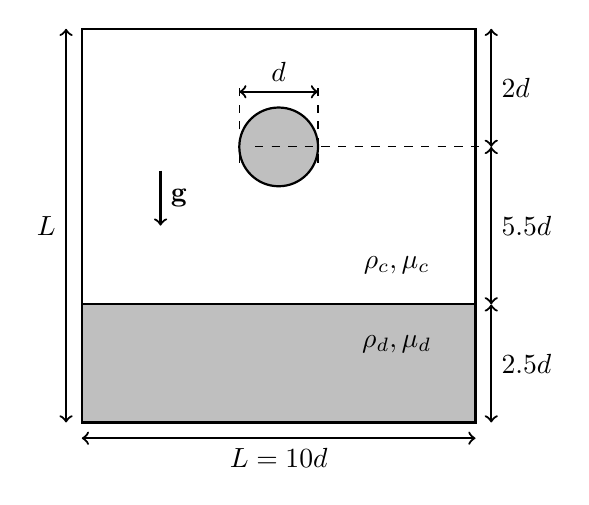
\begin{tikzpicture}[thick]
        \draw (0,0) rectangle (5,5);
        \draw[fill=gray!50] (0,0) rectangle (5,1.5);
        \draw[fill=gray!50] (2.5,3.5) circle (0.5);
        \draw[<->](0,-0.2) --++ (5,0)node[midway,below]{$L  = 10 d$};
        \draw[<->](-0.2,0) --++ (0,5)node[midway,left]{$L$};
        \draw[<->](5.2,0) --++ (0,1.5)node[midway,right]{$2.5 d$};
        \draw[<->](5.2,1.5) --++ (0,2)node[midway,right]{$5.5 d$};
        \draw[<->](5.2,3.5) --++ (0,1.5)node[midway,right]{$ 2d$};
        \draw[dashed,thin](2.2,3.5) --++ (2.9,0);
        \draw[dashed,thin](2.2,3.5) --++ (2.9,0);
        \draw[->](1,3.2) --++ (0,-0.7)node[midway,right]{$\textbf{g}$};
        \draw[<->](2,4.2) --++ (1,0)node[midway,above]{$d$};
        \draw[thin,dashed](2,3.3) --++ (0,1);
        \draw[thin,dashed](3,3.3) --++ (0,1);
        \node (a) at (4,2){$\rho_c, \mu_c$};
        \node (a) at (4,1){$\rho_d, \mu_d$};
    \end{tikzpicture}
    \caption{(left) Scheme of the computational set up at the initial time. (right) picture of the computational domain with the interfaces represented in grey.}
    \label{fig:schemeLong}
\end{figure}
\begin{figure}[h!]
    \centering
    \begin{tikzpicture}
        \node (img1) at (0,0.35\textwidth)             {
\includegraphics[height = 0.3\textwidth]{image/VALIDATION2.0/Longmire/IMG/image-010.png}};
        \node (img2) at (0.35\textwidth,0.35\textwidth) {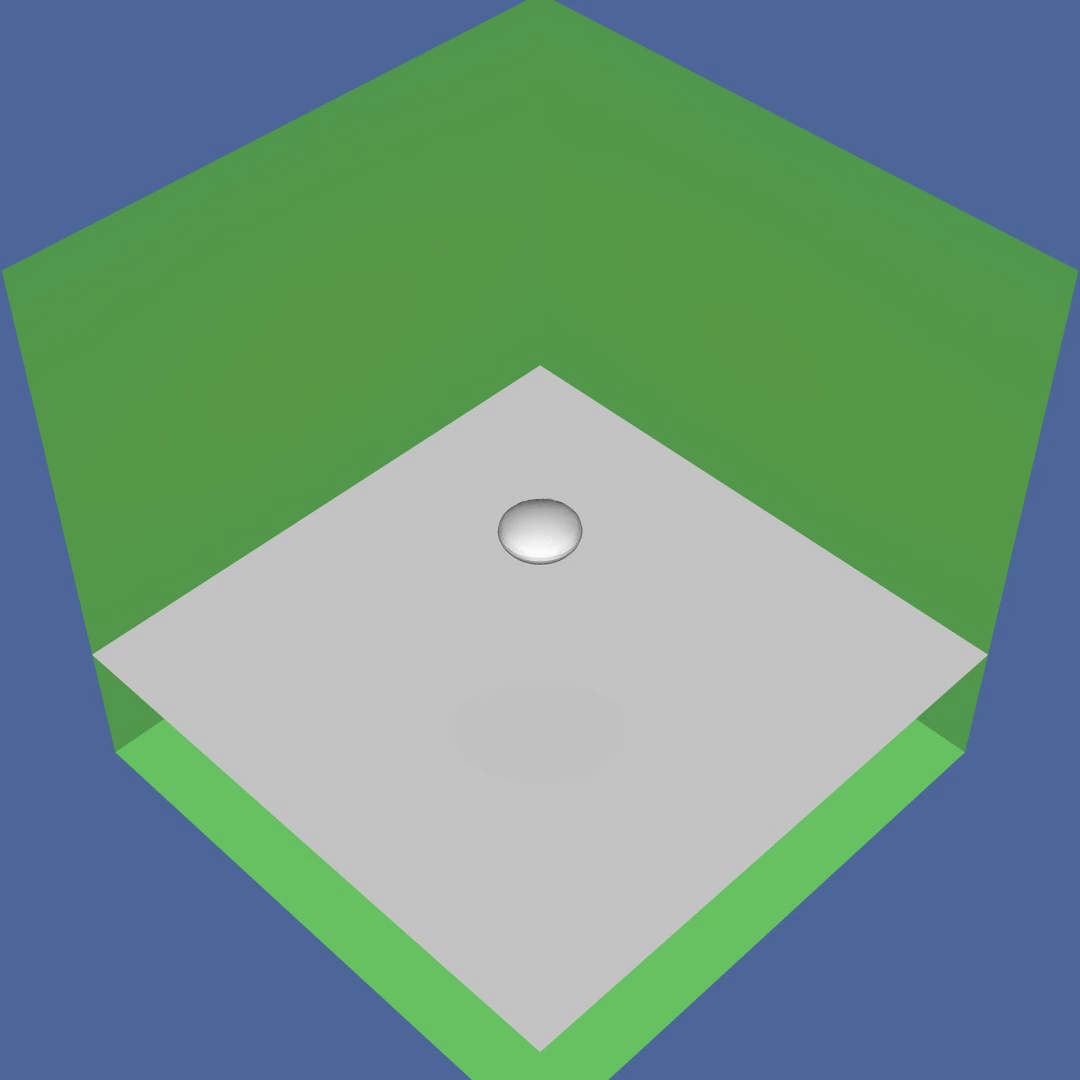
\includegraphics[height = 0.3\textwidth]{image/VALIDATION2.0/Longmire/IMG/image-020.png}};
        \node (img3) at (0.7\textwidth,0.35\textwidth) {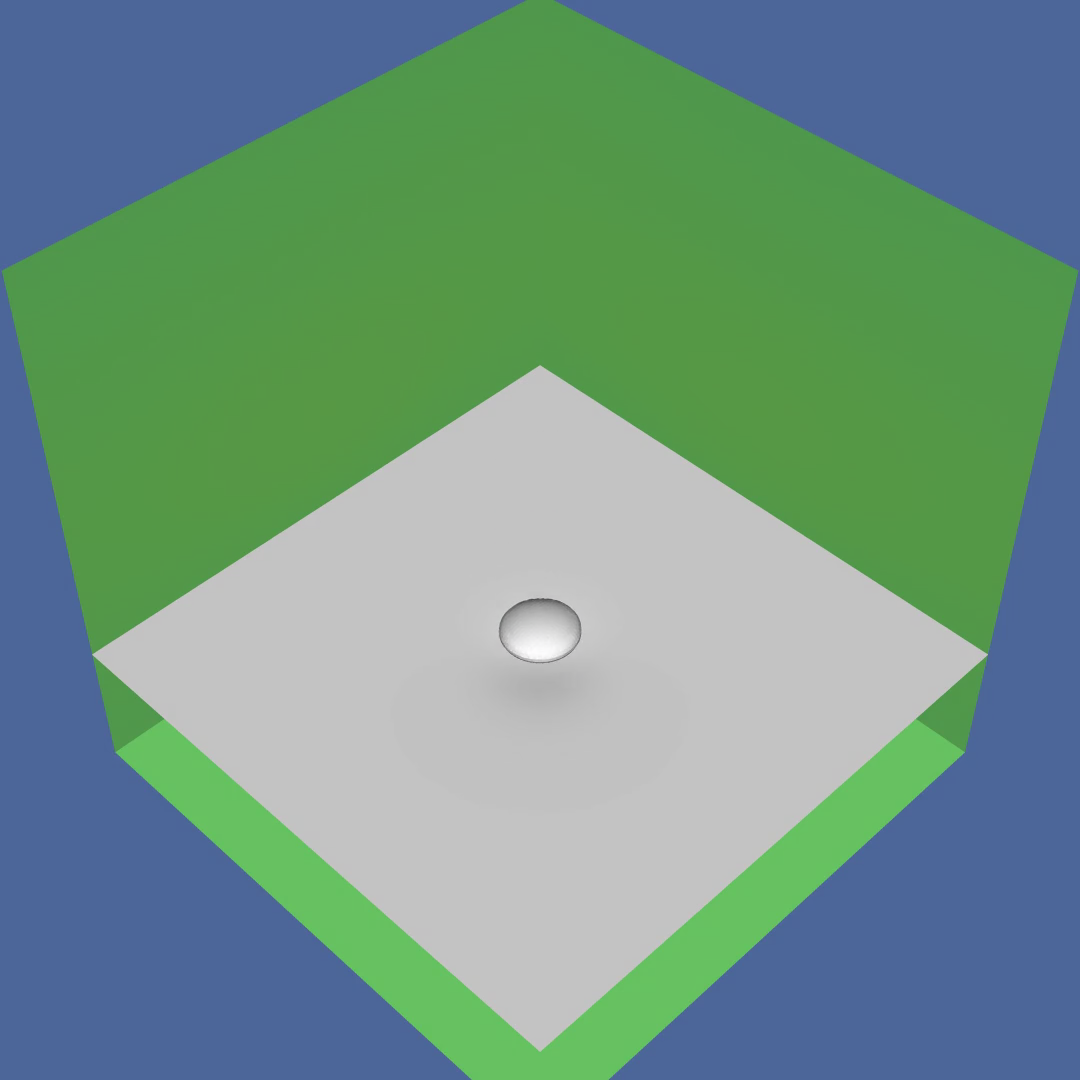
\includegraphics[height = 0.3\textwidth]{image/VALIDATION2.0/Longmire/IMG/image-030.png}};
        \node (img4) at (0,0)                         {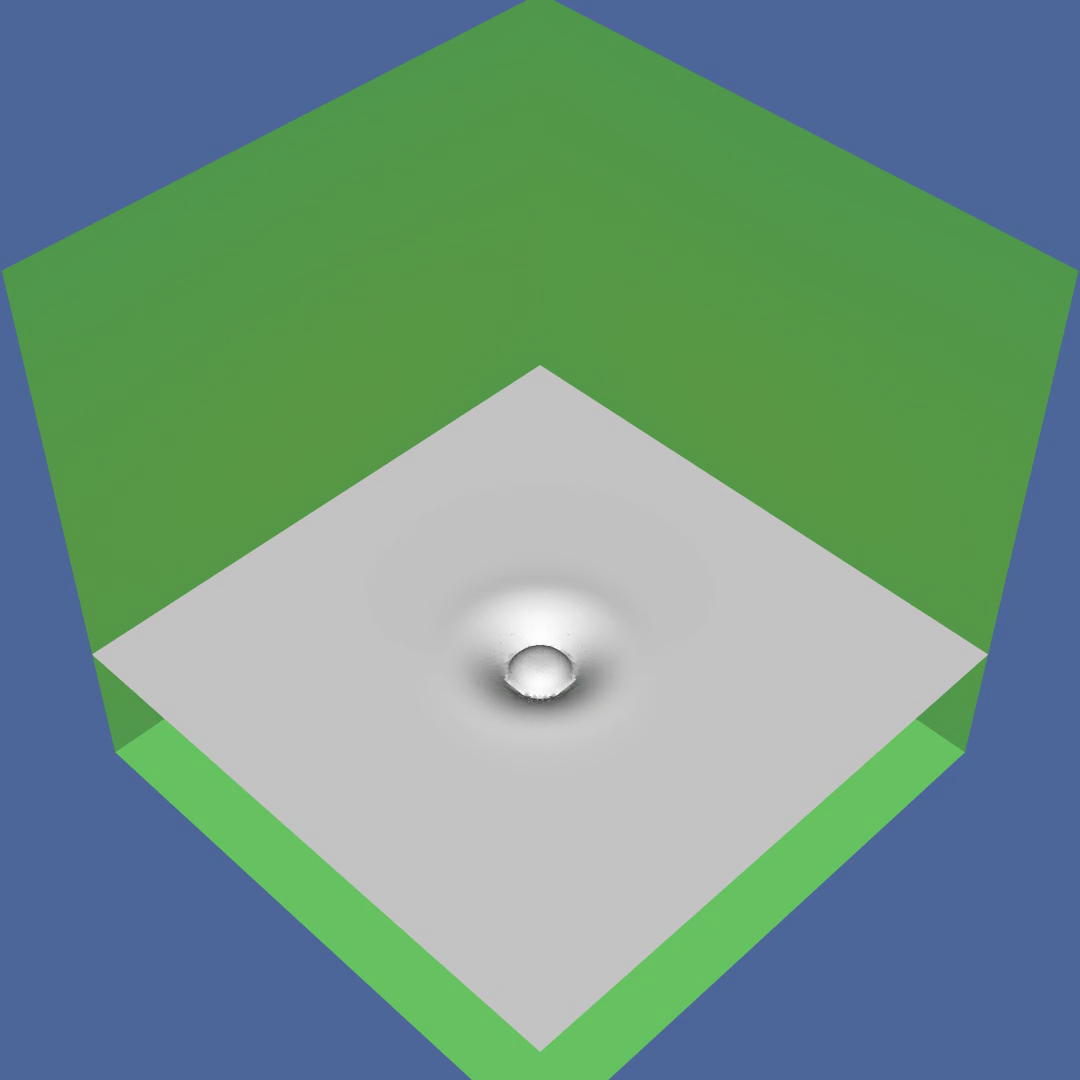
\includegraphics[height = 0.3\textwidth]{image/VALIDATION2.0/Longmire/IMG/image-040.png}};
        \node (img5) at (0.35\textwidth,0)             {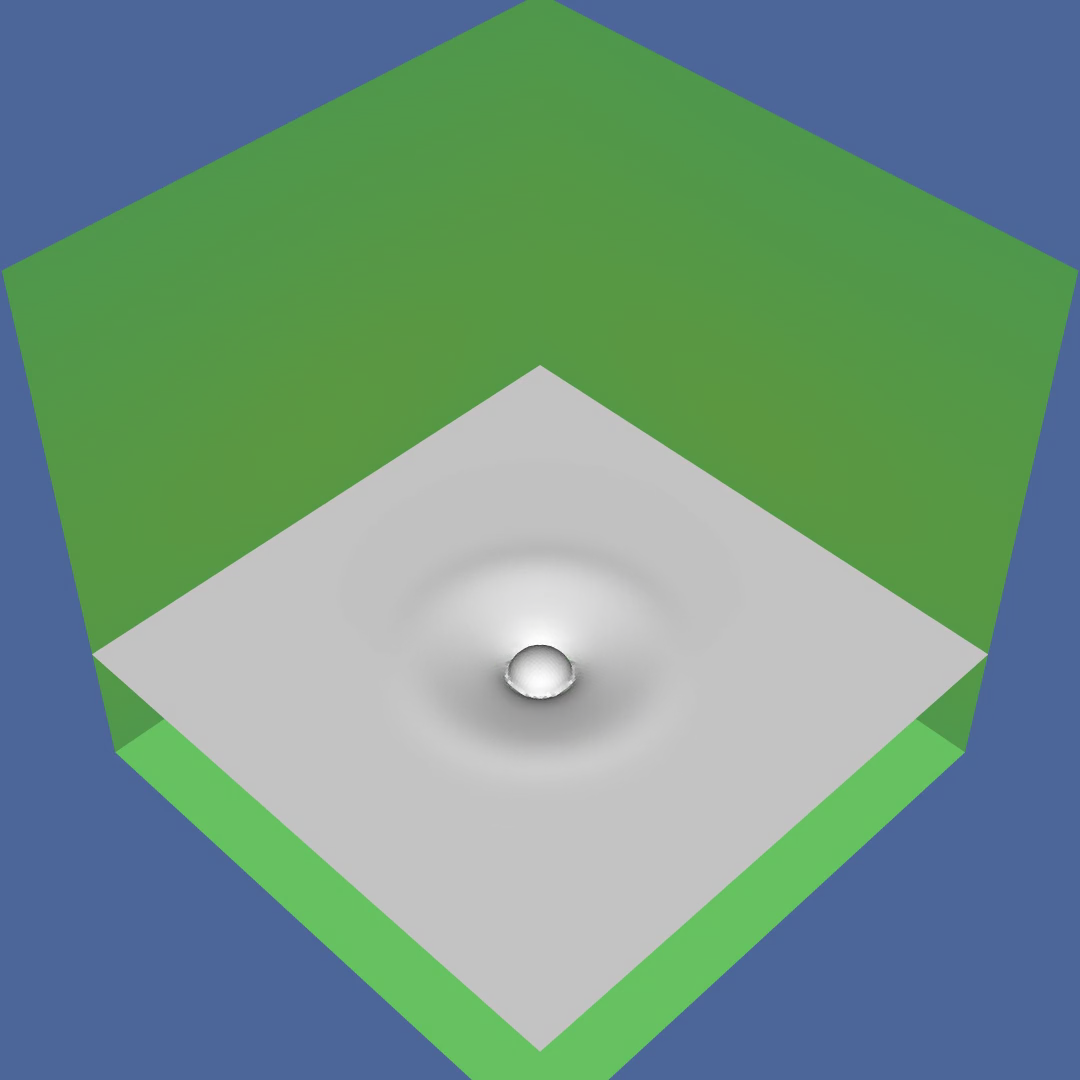
\includegraphics[height = 0.3\textwidth]{image/VALIDATION2.0/Longmire/IMG/image-050.png}};
        \node (img6) at (0.7\textwidth,0)             {
\includegraphics[height = 0.3\textwidth]{image/VALIDATION2.0/Longmire/IMG/image-060.png}};
        \node[below] at (img1.south){$t_i = -5.5$};
        \node[below] at (img2.south){$t_i = -2$};
        \node[below] at (img3.south){$t_i = 0$};
        \node[below] at (img4.south){$t_i = 2.5$};
        \node[below] at (img5.south){$t_i = 5$};
        \node[below] at (img6.south){$t_i = 15$};
    \end{tikzpicture}

    % \centering
    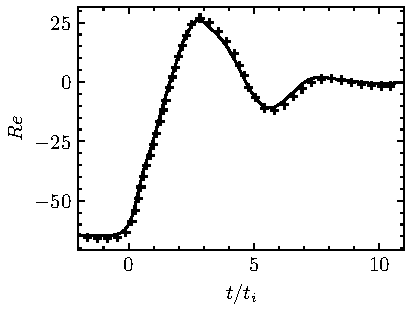
\includegraphics[height = 0.35\textwidth]{image/VALIDATION2.0/Longmire/Re.pdf}
    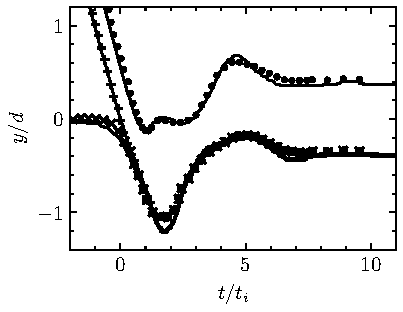
\includegraphics[height = 0.35\textwidth]{image/VALIDATION2.0/Longmire/Dist.pdf}
    \caption{(left) Time evolution of the Reynolds number based on the droplet velocity, $Re(t) = \rho_fU d /\mu_f$ in term of the dimensionless time, (+) numerical results of  \citet{balcazar2015multiple} (right)  position of the interfaces, ($\bullet$) top droplets surface, ($+$) bot droplet surface, (x) pool surface. (Symbols) experimental result of \citet{mohamed2003drop} (solid line) present numerical simulations with $d/\Delta = 30$. }
    \label{fig:resultslong}
\end{figure}
\ref{fig:resultslong} represent the comparison between our results aigainst the experiment of \citet{mohamed2003drop} (right) and the numerical simulation of \citet{balcazar2015multiple} (left). 
From the very good agreement obtained with the numerical and experimental results we conclude that the kinematic is preserved during the contact time for a mesh definition of $d/\Delta = 30$. 

